\titre{}
\theme{derivation}
\auteur{Nathan Scheinmann}
\niveau{3M}
\source{sesamath3e}
\type{serie}
\piments{2}
\pts{}
\annee{2425}

\contenu{
\tcblower
Sur le graphique ci-dessous on a représenté une fonction \(g\) pour \(x\in[-4;5{,}5]\) :
% (graphique)
	\begin{center}
		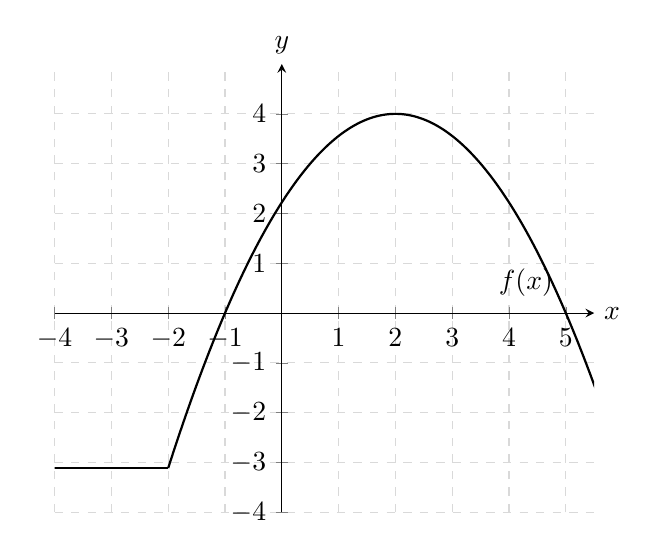
\begin{tikzpicture}
  \begin{axis}[
    axis lines=middle,
    xlabel={$x$}, ylabel={$y$},
    xlabel style={at=(current axis.right of origin), anchor=west},
    ylabel style={at=(current axis.above origin), anchor=south},
    xmin=-4, xmax=5.5, ymin=-4, ymax=5,
    xtick={-4,-3,-2,-1,0,1,2,3,4,5},
    ytick={-4,-3,-2,-1,0,1,2,3,4},
    grid=both,
    grid style={dashed,gray!30},
  ]
    % branche pour x < -1
    \addplot [domain=-5:-2, samples=200, thick]
      {-4/9*(-2+1)*(-2-5)};
    \addplot [domain=-2:6, samples=200, thick]
      {-4/9*(x+1)*(x-5)} node[above left,pos=0.8] {$f(x)$};
  \end{axis}
\end{tikzpicture}
	\end{center}
\begin{tasks}(1)
  \task Recopier ce graphique puis esquisser aussi précisément que possible la représentation graphique de la fonction dérivée \(g'\).
  \task Sur le même repère, mais avec une autre couleur, tracer une courbe \(h\) qui passe par le point \(P(0;-2)\) et telle que \(h'(x)=g(x)\).
\end{tasks}
}
\correction{

}

